
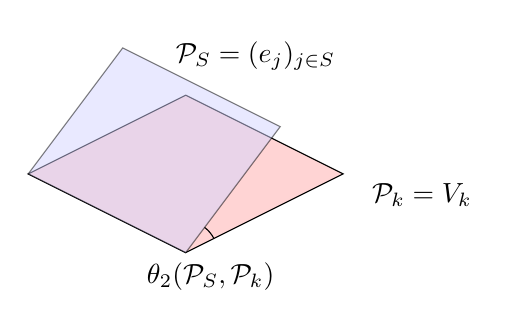
\begin{tikzpicture}[y={(-1cm,0.5cm)},x={(1cm,0.5cm)}, z={(0cm,1cm)}]
\coordinate (A) at (0,0,0);
\coordinate (B) at (2,0,0);
\coordinate (C) at (2.2,1,0);

\draw[fill={rgb:red,1;white,5}] (0,0,0) -- (2,0,0) -- (2,2,0) -- (0,2,0) -- cycle;
\draw[fill={rgb:blue,1;white,5}, opacity=0.5] (0,0,0) -- (2.2,1,0) -- (2.2,3,0) -- (0,2,0) -- cycle;

\begin{scope}
	\draw (0,-1.3,0) node[above left = 0.5mm] {$\theta_{2}(\mathcal{P}_{S},\mathcal{P}_{k})$};
	\draw (2.5,-0.5,0) node[below ] {$\mathcal{P}_{k} = \Span \bm{V}_{k}$};
	\draw (2.7,3,0) node[below right=0.5mm] {$\mathcal{P}_{S} = \Span (e_{j})_{j \in S}$};
    \clip (C) -- (A) -- (B) -- cycle;
    \draw[-] circle[at=(A),radius=4mm];
\end{scope}
% \begin{scope}[->]
% \draw[->] (0,0,0)--(0,0.7*1,0);
% \end{scope}
% \begin{scope}[->]
% \draw[->] (0,0,0)--(0.7*1,0,0);
% \end{scope}
% \begin{scope}[->]
% \draw[->] (0,0,0)--(2.2/2.41,1/2.41,0);
% \end{scope}
% \draw (-0.3,1,0) node[below] {$\tiny \bm{a}_{1} = \bm{b}_{1}$};
% \draw (1,0,0) node[below] {$\tiny \bm{a}_{2}$};
% \draw (1.5*2.2/2.41,1.5*1/2.41,0) node[below] {$\tiny \bm{b}_{2}$};
% \begin{scope}[canvas is yz plane at x=1.25]
% \draw[fill={rgb:blue,1;white,5}] (0,0) -- (2,0) -- (2,2) -- (0,2) -- cycle;
% \end{scope}
\end{tikzpicture}